% ===================================================================
%  Week 16 — Transfer Learning & the DocScan Capstone
% ===================================================================
\documentclass[10pt,aspectratio=169]{beamer}
% ===================================================================
%  Shared Beamer preamble for "Practical Image Processing"
%  English slides. Compile with pdfLaTeX.
% ===================================================================

\usetheme{metropolis}
\usepackage[T1]{fontenc}
\usepackage[utf8]{inputenc}
\usepackage{lmodern}
\usepackage{listings}
\usepackage{tcolorbox}
\usepackage{fontawesome5}
\usepackage{booktabs}
\usepackage{amsmath,amssymb}
\usepackage{tikz}
\usepackage{pgfplots}
\pgfplotsset{compat=1.17}
\usetikzlibrary{arrows.meta,positioning,shapes.geometric,fit,backgrounds,matrix}
\tcbuselibrary{skins,breakable}

% ---- Palette --------------------------------------------------------
\definecolor{coursePrimary}{HTML}{1B4965}   % deep blue
\definecolor{courseAccent}{HTML}{E76F51}    % coral
\definecolor{courseGood}{HTML}{2A9D8F}      % teal
\definecolor{courseBad}{HTML}{C0392B}       % red
\definecolor{courseInfo}{HTML}{2980B9}      % blue
\definecolor{codeBg}{HTML}{F5F6FA}
\definecolor{codeKw}{HTML}{8E44AD}
\definecolor{codeStr}{HTML}{2A9D8F}
\definecolor{codeCom}{HTML}{7F8C8D}

\setbeamercolor{frametitle}{bg=coursePrimary}
\setbeamercolor{progress bar}{fg=courseAccent}
\setbeamercolor{alerted text}{fg=courseAccent}
\metroset{block=fill,sectionpage=progressbar,numbering=fraction}

% ---- Code listings (Python is built into listings) -----------------
\lstdefinestyle{course}{
  backgroundcolor=\color{codeBg},
  basicstyle=\ttfamily\scriptsize,
  keywordstyle=\color{codeKw}\bfseries,
  stringstyle=\color{codeStr},
  commentstyle=\color{codeCom}\itshape,
  numberstyle=\tiny\color{codeCom},
  numbers=left, numbersep=6pt,
  showstringspaces=false, breaklines=true, breakatwhitespace=true,
  tabsize=4, columns=fullflexible,
  frame=single, framesep=4pt, rulecolor=\color{gray!30},
  keepspaces=true, upquote=true, language=Python,
}
\lstset{style=course}
\lstdefinelanguage{bash}{
  keywords={cd,pip,python,venv,source,import}, sensitive=true,
  morecomment=[l]{\#}, morestring=[b]', morestring=[b]",
}

% ---- Reusable callout boxes ----------------------------------------
\newtcolorbox{goodbox}[1][Good practice]{colback=courseGood!8,colframe=courseGood,
  fonttitle=\bfseries,title={\faCheck~#1},boxrule=0.6pt,left=4pt,right=4pt,top=3pt,bottom=3pt}
\newtcolorbox{badbox}[1][Pitfall]{colback=courseBad!8,colframe=courseBad,
  fonttitle=\bfseries,title={\faTimes~#1},boxrule=0.6pt,left=4pt,right=4pt,top=3pt,bottom=3pt}
\newtcolorbox{infobox}[1][Note]{colback=courseInfo!8,colframe=courseInfo,
  fonttitle=\bfseries,title={\faInfoCircle~#1},boxrule=0.6pt,left=4pt,right=4pt,top=3pt,bottom=3pt}
\newtcolorbox{mathbox}[1][Math]{colback=coursePrimary!6,colframe=coursePrimary,
  fonttitle=\bfseries,title={\faCalculator~#1},boxrule=0.6pt,left=4pt,right=4pt,top=3pt,bottom=3pt}

\newcommand{\keyidea}[1]{\begin{alertblock}{Key idea}#1\end{alertblock}}
\newcommand{\term}[1]{\textbf{\color{coursePrimary}#1}}
\newcommand{\code}[1]{\lstinline[basicstyle=\ttfamily\small]|#1|}

% ---- A helper to draw a small pixel grid, cells shaded by value ----
% \pixelgrid{ {10,20,120,200,240}, {30,60,130,180,230}, ... }
\newcommand{\pixelgrid}[1]{%
  \begin{tikzpicture}[font=\scriptsize,scale=0.6]
    \foreach \row [count=\ry] in {#1} {
      \foreach \val [count=\cx] in \row {
        \draw[gray,fill=coursePrimary!8] (\cx,-\ry) rectangle ++(1,-1);
        \node at (\cx+0.5,-\ry-0.5) {\val};
      }
    }
  \end{tikzpicture}}


\title{Transfer Learning \& the DocScan Capstone}
\subtitle{Week 16 — Standing on a giant's shoulders, and shipping the project}
\author{Practical Image Processing}
\date{Lecture 16 \textbullet\ 60--70 min}

\begin{document}

\maketitle

\begin{frame}{The finale}
  \begin{columns}[T]
    \begin{column}{0.58\textwidth}
      \begin{itemize}
        \item Week 12: HOG+SVM plateaued at \textbf{0.48} on look-alike cars.
        \item Week 13: CNNs learn features — but need lots of data.
        \item \alert{Today:} \term{transfer learning} — reuse a net trained on millions of images —
              and assemble the whole \term{DocScan} pipeline.
      \end{itemize}
    \end{column}
    \begin{column}{0.42\textwidth}
      \begin{alertblock}{Today's real result}
        Same cars, same SVM, but \term{deep features} from a pretrained net:
        \textbf{0.48 $\rightarrow$ 0.87}.
      \end{alertblock}
    \end{column}
  \end{columns}
\end{frame}

\begin{frame}{Roadmap}\tableofcontents\end{frame}

% ==================================================================
\section{The small-data problem}
% ==================================================================

\begin{frame}{Why we can't just train a big CNN}
  \begin{itemize}
    \item Deep CNNs have millions of parameters and need $10^4$--$10^6$ labelled images.
    \item We have 60 images per car model — training a big net from scratch would badly overfit.
    \item Yet the HOG ceiling (0.48) shows hand features aren't enough. What now?
  \end{itemize}
  \keyidea{Most real projects have \emph{small} data. Transfer learning is how you still use deep learning.}
\end{frame}

\begin{frame}{The key insight}
  \begin{itemize}
    \item A CNN trained on ImageNet (1.2M images, 1000 classes) learned \emph{general} visual features:
          edges, textures, shapes, parts.
    \item Those early/mid features are useful for \emph{almost any} image task — including cars.
    \item So: \term{reuse} those learned features instead of learning them from scratch.
  \end{itemize}
  \keyidea{The first layers of a good vision net are a general-purpose feature extractor. Don't waste them.}
\end{frame}

% ==================================================================
\section{Transfer learning}
% ==================================================================

\begin{frame}{Two flavours of transfer learning}
  \begin{center}
  \begin{tabular}{@{}lll@{}}
    \toprule
    \textbf{Approach} & \textbf{What you do} & \textbf{When} \\
    \midrule
    Feature extraction & freeze the net, train a new classifier head & very small data \\
    Fine-tuning & unfreeze some top layers, train them too & more data \\
    \bottomrule
  \end{tabular}
  \end{center}
  \begin{itemize}
    \item We use \term{feature extraction}: a frozen ImageNet ConvNeXt turns each car into a 1024-D vector,
          then an SVM classifies — exactly Week 12's classifier, better features.
  \end{itemize}
\end{frame}

\begin{frame}{Our result: the ceiling lifts}
  \begin{columns}[T]
    \begin{column}{0.5\textwidth}\begin{center}
      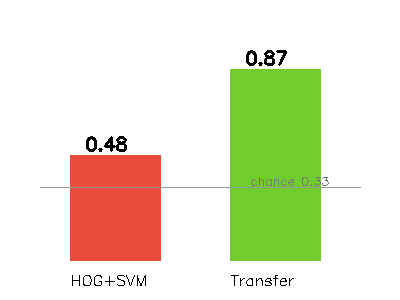
\includegraphics[width=0.95\linewidth]{../assets/accuracy_bars.png}
    \end{center}\end{column}
    \begin{column}{0.5\textwidth}
      \begin{itemize}
        \item \textbf{Same} 180 images, \textbf{same} SVM, \textbf{same} split.
        \item Only change: HOG $\rightarrow$ frozen ImageNet features.
        \item 0.48 $\rightarrow$ \textbf{0.87}. The features were the bottleneck all along.
      \end{itemize}
    \end{column}
  \end{columns}
\end{frame}

\begin{frame}{Confusion matrix after transfer}
  \begin{columns}[T]
    \begin{column}{0.5\textwidth}\begin{center}
      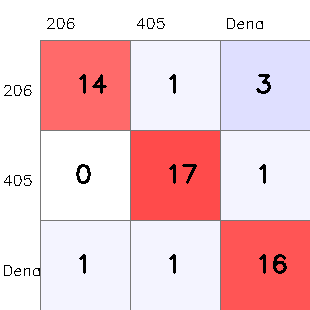
\includegraphics[width=0.95\linewidth]{../assets/confusion_transfer.png}
    \end{center}\end{column}
    \begin{column}{0.5\textwidth}
      \begin{itemize}
        \item The diagonal is now dominant — most cars classified correctly.
        \item Compare to Week 12's near-random confusion matrix.
        \item The pretrained net ``sees'' the fine differences HOG missed.
      \end{itemize}
    \end{column}
  \end{columns}
\end{frame}

\begin{frame}{Why this works so well}
  \begin{itemize}
    \item ImageNet includes many vehicles — the net already learned car-relevant parts.
    \item Its mid-level features (grille shapes, light patterns) are exactly what separates models.
    \item We get the power of a huge net with only 60 images per class and seconds of training.
  \end{itemize}
  \begin{goodbox}
    Transfer learning is the single most useful deep-learning technique for real, small-data projects.
  \end{goodbox}
\end{frame}

\begin{frame}{What each layer transfers}
  \begin{itemize}
    \item \term{Early layers}: edges, colours, textures — universal, transfer to \emph{any} task.
    \item \term{Middle layers}: parts and motifs — transfer well to related domains.
    \item \term{Late layers}: class-specific (``golden retriever'') — least transferable; often replaced.
  \end{itemize}
  \keyidea{The more your task differs from ImageNet, the more late layers you should retrain.}
\end{frame}

\begin{frame}{The domain gap}
  \begin{itemize}
    \item ImageNet is natural photos. If your images are very different (X-rays, thermal, tiny digits),
          the transfer is weaker.
    \item Meters and cars are ordinary photos $\rightarrow$ the gap is small $\rightarrow$ transfer works great (our 0.87).
    \item Larger gap $\rightarrow$ fine-tune more layers, or find a model pretrained on closer data.
  \end{itemize}
  \begin{mathbox}
    Rule of thumb: small gap + small data $\rightarrow$ freeze \& extract; large gap + more data $\rightarrow$ fine-tune.
  \end{mathbox}
\end{frame}

\begin{frame}{Data augmentation for small data}
  \begin{itemize}
    \item Multiply your data for free: random flips, small rotations, brightness/contrast jitter, crops.
    \item Each variant teaches the same label under a new nuisance $\rightarrow$ more invariance, less overfitting.
    \item Especially valuable when combined with transfer learning on tiny datasets.
  \end{itemize}
  \begin{goodbox}
    Augmentation is the cheapest accuracy you will ever buy — always try it on small-data problems.
  \end{goodbox}
\end{frame}

\begin{frame}{Practical transfer-learning tips}
  \begin{itemize}
    \item Use the pretrained model's \emph{own} preprocessing (resize, normalize) — mismatch hurts a lot.
    \item Start with \term{feature extraction}; only fine-tune if you have enough data and need more.
    \item Freeze early layers (general), fine-tune late layers (task-specific) if you do fine-tune.
    \item Watch for overfitting — small data still bites; use augmentation and regularization.
  \end{itemize}
\end{frame}

% ==================================================================
\section{The DocScan capstone}
% ==================================================================

\begin{frame}{DocScan: the whole course in one pipeline}
  \begin{columns}[T]
    \begin{column}{0.34\textwidth}\begin{center}
      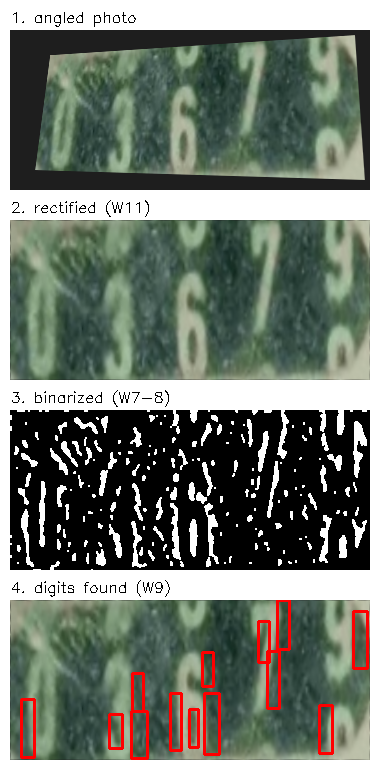
\includegraphics[height=0.82\textheight]{../assets/docscan_pipeline.png}
    \end{center}\end{column}
    \begin{column}{0.66\textwidth}
      \begin{itemize}
        \item \textbf{1. Photo} — a meter snapped at an angle (raw input).
        \item \textbf{2. Rectify} (W11) — homography warps it flat.
        \item \textbf{3. Binarize} (W2/7/8) — threshold + morphology clean it.
        \item \textbf{4. Segment} (W9) — contours find each digit box.
        \item \textbf{5. Read} (W13) — a CNN classifies each digit $\rightarrow$ ``03679''.
      \end{itemize}
    \end{column}
  \end{columns}
\end{frame}

\begin{frame}{Every week was a stage}
  \begin{center}
  \begin{tabular}{@{}ll@{}}
    \toprule
    \textbf{Weeks} & \textbf{DocScan role} \\
    \midrule
    1--4 Pixels, histograms, filtering, denoise & clean the raw photo \\
    5--6 Edges, Fourier & find structure, remove periodic noise \\
    7--9 Morphology, segmentation, contours & isolate the digits \\
    10--11 Features, homography & rectify to a flat scan \\
    12--16 ML, CNNs, transfer learning & read the digits \\
    \bottomrule
  \end{tabular}
  \end{center}
  \keyidea{DocScan isn't a separate project — it's the spine that every week added a vertebra to.}
\end{frame}

\begin{frame}{Engineering a robust pipeline}
  \begin{itemize}
    \item \term{Confidence gates}: if RANSAC inliers are too few, ask for a new photo (don't guess).
    \item \term{Sanity checks}: a meter reading has a fixed number of digits — reject wrong counts.
    \item \term{Fallbacks}: if the feature path fails, try the contour path (and vice-versa).
    \item \term{Logging}: record per-stage quality (RMSE, digit confidences) to debug failures.
  \end{itemize}
  \begin{badbox}
    A demo works on one clean image; a product survives blur, glare, tilt, and dirt. Design for failure.
  \end{badbox}
\end{frame}

% ==================================================================
\section{In-class exercise}
% ==================================================================

\begin{frame}{\faPen~In-class exercise (10 min)}
  \begin{infobox}[Design decisions]
  \end{infobox}
  \begin{enumerate}
    \item You have 40 images per class. From-scratch CNN or transfer learning? Why?
    \item Transfer learning lifted cars 0.48$\rightarrow$0.87 with the \emph{same} SVM. What changed, exactly?
    \item In DocScan, the rectify step returns very few RANSAC inliers. What should the system do?
  \end{enumerate}
\end{frame}

\begin{frame}{\faPen~Debrief}
  \begin{itemize}
    \item (1) \term{Transfer learning} — 40 images is far too few to train a deep net from scratch without overfitting.
    \item (2) Only the \term{features}: hand-designed HOG $\rightarrow$ pretrained deep features. The classifier was identical.
    \item (3) \term{Gate it}: treat the rectification as unreliable and prompt for a new photo rather than reading a bad scan.
  \end{itemize}
  \keyidea{Good ML engineering is mostly good \emph{features} and honest \emph{failure handling} — not fancier models.}
\end{frame}

% ==================================================================
\section{Course wrap-up}
% ==================================================================

\begin{frame}{The arc of the course}
  \begin{itemize}
    \item We started with a single pixel and ended with a pretrained neural network.
    \item Classical IP (weeks 1--11): precise, interpretable, no training — still essential for geometry \& cleanup.
    \item Learning (weeks 12--16): powerful for recognition, especially via transfer learning.
    \item \alert{A real system uses both}: classical to prepare, learned to recognize.
  \end{itemize}
\end{frame}

\begin{frame}{Choosing the right tool}
  \begin{center}
  \begin{tabular}{@{}ll@{}}
    \toprule
    \textbf{If you need to\ldots} & \textbf{Reach for\ldots} \\
    \midrule
    align/rectify/measure geometry & classical (homography, contours) \\
    clean noise, threshold, morphology & classical filters \\
    recognize with small data & transfer learning \\
    recognize with big data & train/fine-tune a CNN \\
    \bottomrule
  \end{tabular}
  \end{center}
  \keyidea{The mark of an engineer: picking the simplest tool that solves the problem reliably.}
\end{frame}

\begin{frame}{Honesty, ethics, and limits}
  \begin{itemize}
    \item Report the \emph{test} number, the failure cases, and the data you trained on — not just the best demo.
    \item A misread meter digit is a wrong bill; know your error rate and gate low-confidence reads.
    \item Beware dataset bias: if all training meters are clean and bright, expect failure on dirty ones.
  \end{itemize}
  \begin{badbox}
    ``97\% accurate'' means nothing without: on what data, which metric, and how it fails.
  \end{badbox}
\end{frame}

\begin{frame}{A quick self-check on the whole course}
  \begin{itemize}
    \item Can you clean a noisy image (denoise, threshold, morphology)? (W1--8)
    \item Can you find and measure shapes/contours? (W9)
    \item Can you rectify a tilted photo with a homography? (W10--11)
    \item Can you build a features$\rightarrow$classifier and a CNN, and use transfer learning? (W12--16)
  \end{itemize}
  \keyidea{If yes to all four, you can build the majority of practical vision systems end to end.}
\end{frame}

\begin{frame}{Where to go next}
  \begin{itemize}
    \item \term{Detection} (YOLO, Faster-RCNN): find \emph{and} locate objects — the next step past classification.
    \item \term{Segmentation} (U-Net, SAM): label every pixel — for your power-line/mask datasets.
    \item \term{OCR} systems (Tesseract, TrOCR): full text reading pipelines built on these ideas.
    \item \term{Deployment}: on-device (TFLite, ONNX), latency, and robustness in the field.
  \end{itemize}
\end{frame}

\begin{frame}{The capstone deliverable}
  \begin{alertblock}{Final project (see \code{capstone/})}
    \begin{enumerate}
      \item Assemble the full DocScan pipeline on real \code{E:/data} images.
      \item Rectify (W11) $\rightarrow$ clean/segment (W7--9) $\rightarrow$ read digits (W13 or transfer).
      \item Add at least two robustness features (confidence gate, digit-count check, fallback).
      \item Report end-to-end accuracy and where it fails; propose one concrete improvement.
    \end{enumerate}
  \end{alertblock}
\end{frame}

\begin{frame}[standout]
  From one pixel to a working scanner.\\[4pt]
  \normalsize Classical vision to prepare, deep learning to recognize — and the judgment to know which, when.
\end{frame}

\end{document}
